\section{Zielsetzung}
Untersuchung einer Wärmepumpe und ermittlung der Qualität dieser.
\section{Theorie}
\label{sec:Theorie}

Der zweite Hauptsatz der Thermodynamik besagt, dass Wärmeenergie vom wärmeren in das kältere Reservoir fließt.
Damit sich die Flussrichtung der WäWärmeenergie ändert muss beispielsweise mechanische Arbeit aufgewendet werden.
Eine Apparatur, welche dieses vollführt, ist die Wärmepume.
Die Güteziffer

\begin{equation}
	\label{eq:gl1}
	\nu=\frac{Q_1}{A}
\end{equation}

beschreibt das Verhältnis zwischen transportierter Wärmemenge und verrichteter Arbeit.
Mit dem zweiten Hauptsatz der Thermodynamik lässt sich nun folgende Aussage über über Wärmemengen der beiden Reservoirs und Temperaturen dieser treffen:
\begin{equation}
		\label{eq:gl2}
	\frac{Q_1}{T_1}-\frac{Q_2}{T_2}=0.
\end{equation}
Dies gilt jedoch nur unter idealisierten den Bedingungen, dass der Prozess reversibel ist.
Hieraus lässt sich für die Güteziffer die Beziehung
\begin{equation}
	\nu_{\text{id}}=\frac{T_1}{T_1-T_2}
	\label{eq:guetezifferideal}
\end{equation}
folgern.
Die reale Wärmepumpe kann diese forderung jedoch nicht erfüllen.
Für den realen, irreversiblen Fall gilt
\begin{equation}
		\label{eq:gl3}
	\frac{Q_1}{T_1}-\frac{Q_2}{T_2}>0 .
\end{equation}
Daraus lässt sich folgern, dass die Wärmepumpe um so günstiger arbeitet je kleiner die Temperaturdifferenz zwischen den Wärmereservoirs ist.
\subsection{Aufbau der Wärmepumpe}
\label{sec:AdW}
In Abbildung \ref{fig:aufbau} wird der Aufbau einer Wärmepumpe dargestellt.
Innerhalb eines geschlossenen Systems verdampft und kondensiert ein reales Gas in den verschiedenen Wärmereservoirs.
Dies wird durch Druckunterschiede in den Wärmeresrvoirs realisiert.
Das Gas wird komprimiert wodurch es kondensiert und Wärme an das Reservoir 1 abgibt.
Das Transportmedium durchläuft das Drosselventil D und geht in dem Reservoir 2 in Gasform über.
Hierbei entzieht es Reservoir 2 Wärme.
In dem flüssigen Zustand wird das Transportmedium von Gasresten mittels eines "Reinigers" befreit, um das Drosselventil nicht zu beschädigen.
\begin{figure}[H]
    \centering
    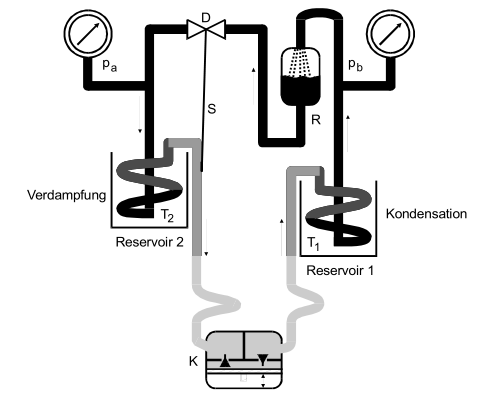
\includegraphics[width=\textwidth]{content/aufbau.png}
    \caption{Aufbau der Wärmepumpe}
    \label{fig:aufbau}
\end{figure}
\subsection{Bestimmung der Kenngrößen}
\label{sec:BdK}
Die Güteziffer, der Massendurchsatz des Transportmediums und Wirkungsgrad des Kompressors sind in diesem Versuch die Interessanten Kenngrößen.
Die pro Zeiteinheit gewonnene Wärmemenge berechnet sich nach:
\begin{equation}
	\frac{dQ_1}{dt}=(m_1c_{\text{w}}+m_{\text{k}}c_{\text{k}})\cdot \frac{dT_1}{dt} .
	\label{eq:gueteziffer}
\end{equation}
Hierbei sind $c_{\text{w}}$ und $c_{\text{w}}$ die Wärekapazität des Wassers und der Apparatur.
Mit der Leistungsaufnahme $N$ lässt sich die Güteziffer durch
\begin{equation}
	\nu=\frac{dQ_1}{dt N}
\end{equation}
beschreiben.
Analog zu \eqref{eq:gueteziffer} lässt sich die entnommene Wärmemenge $Q_2$ pro Zeiteinheit bestimmen.
Ist die Verdampfungswärme $L$ bekannt kann der Massendurchsatz
\begin{equation}
	\frac{dQ_2}{dt}=L\frac{dm}{dt}
	\label{eq:massendurchsatz}
\end{equation}
berechnet werden.
Die mechanische Kompressorleistung berechnet sich über:
\begin{equation}
	N_{\text{mech}} = \frac{1}{\kappa - 1} \left( p_{\text{b}} \sqrt[\kappa]{\frac{p_{\text{a}}}{p_{\text{b}}}} -p_{\text{a}} \right) \frac{1}{\rho} \cdot \frac{dm}{dt} .
	\label{eq:arbeit}
\end{equation}
Wobei $\rho$ die Dichte des Transportmediums bezeichnet.
